
% Template for Elsevier CRC journal article
% version 1.1 dated 16 March 2010

% This file (c) 2010 Elsevier Ltd.  Modifications may be freely made,
% provided the edited file is saved under a different name

% This file contains modifications for Procedia Computer Science
% but may easily be adapted to other journals

% Changes since version 1.0
% - elsarticle class option changed from 1p to 3p (to better reflect CRC layout)

%-----------------------------------------------------------------------------------

%% This template uses the elsarticle.cls document class and the extension package ecrc.sty
%% For full documentation on usage of elsarticle.cls, consult the documentation "elsdoc.pdf"
%% Further resources available at http://www.elsevier.com/latex

%-----------------------------------------------------------------------------------

%%%%%%%%%%%%%%%%%%%%%%%%%%%%%%%%%%%%%%%%%%%%%%
%%%%%%%%%%%%%%%%%%%%%%%%%%%%%%%%%%%%%%%%%%%%%%
%%                                          %%
%% Important note on usage                  %%
%% -----------------------                  %%
%% This file must be compiled with PDFLaTeX %%
%% Using standard LaTeX will not work!      %%
%%                                          %%
%%%%%%%%%%%%%%%%%%%%%%%%%%%%%%%%%%%%%%%%%%%%%%
%%%%%%%%%%%%%%%%%%%%%%%%%%%%%%%%%%%%%%%%%%%%%%

%% The '3p' and 'times' class options of elsarticle are used for Elsevier CRC
\documentclass[3p,times,twocolumn]{elsarticle}

%% The `ecrc' package must be called to make the CRC functionality available
\usepackage{ecrc}
\usepackage{lipsum}
\usepackage[sort, numbers]{natbib}

%% The ecrc package defines commands needed for running heads and logos.
%% For running heads, you can set the journal name, the volume, the starting page and the authors

%% set the volume if you know. Otherwise `00'
\volume{00}

%% set the starting page if not 1
\firstpage{1}

%% Give the name of the journal
\journalname{Software Development for Engineering Research}

%% Give the author list to appear in the running head
%% Example \runauth{C.V. Radhakrishnan et al.}
\runauth{}

%% The choice of journal logo is determined by the \jid and \jnltitlelogo commands.
%% A user-supplied logo with the name <\jid>logo.pdf will be inserted if present.
%% e.g. if \jid{yspmi} the system will look for a file yspmilogo.pdf
%% Otherwise the content of \jnltitlelogo will be set between horizontal lines as a default logo

%% Give the abbreviation of the Journal.
\jid{SDER}

%% Give a short journal name for the dummy logo (if needed)
\jnltitlelogo{}

%% Hereafter the template follows `elsarticle'.
%% For more details see the existing template files elsarticle-template-harv.tex and elsarticle-template-num.tex.

%% Elsevier CRC generally uses a numbered reference style
%% For this, the conventions of elsarticle-template-num.tex should be followed (included below)
%% If using BibTeX, use the style file elsarticle-num.bst

%% End of ecrc-specific commands
%%%%%%%%%%%%%%%%%%%%%%%%%%%%%%%%%%%%%%%%%%%%%%%%%%%%%%%%%%%%%%%%%%%%%%%%%%

%% The amssymb package provides various useful mathematical symbols
\usepackage{amssymb}
%% The amsthm package provides extended theorem environments
%% \usepackage{amsthm}

%% The lineno packages adds line numbers. Start line numbering with
%% \begin{linenumbers}, end it with \end{linenumbers}. Or switch it on
%% for the whole article with \linenumbers after \end{frontmatter}.
%% \usepackage{lineno}

%% natbib.sty is loaded by default. However, natbib options can be
%% provided with \biboptions{...} command. Following options are
%% valid:

%%   round  -  round parentheses are used (default)
%%   square -  square brackets are used   [option]
%%   curly  -  curly braces are used      {option}
%%   angle  -  angle brackets are used    <option>
%%   semicolon  -  multiple citations separated by semi-colon
%%   colon  - same as semicolon, an earlier confusion
%%   comma  -  separated by comma
%%   numbers-  selects numerical citations
%%   super  -  numerical citations as superscripts
%%   sort   -  sorts multiple citations according to order in ref. list
%%   sort&compress   -  like sort, but also compresses numerical citations
%%   compress - compresses without sorting
%%
%% \biboptions{comma,round}

% \biboptions{}

% if you have landscape tables
\usepackage[figuresright]{rotating}


\usepackage{graphicx}
\graphicspath{{./figures/}}
\DeclareGraphicsExtensions{.PNG}
\bibliographystyle{elsarticle-num}
% put your own definitions here:
%   \newcommand{\cZ}{\cal{Z}}
%   \newtheorem{def}{Definition}[section]
%   ...

% add words to TeX's hyphenation exception list
%\hyphenation{author another created financial paper re-commend-ed Post-Script}

% declarations for front matter

\begin{document}

\begin{frontmatter}

%% Title, authors and addresses

%% use the tnoteref command within \title for footnotes;
%% use the tnotetext command for the associated footnote;
%% use the fnref command within \author or \address for footnotes;
%% use the fntext command for the associated footnote;
%% use the corref command within \author for corresponding author footnotes;
%% use the cortext command for the associated footnote;
%% use the ead command for the email address,
%% and the form \ead[url] for the home page:
%%
%% \title{Title\tnoteref{label1}}
%% \tnotetext[label1]{}
%% \author{Name\corref{cor1}\fnref{label2}}
%% \ead{email address}
%% \ead[url]{home page}
%% \fntext[label2]{}
%% \cortext[cor1]{}
%% \address{Address\fnref{label3}}
%% \fntext[label3]{}

\dochead{}
%% Use \dochead if there is an article header, e.g. \dochead{Short communication}

\title{StoveOpt: Biomass Cookstove Optimization Tool}

%% use optional labels to link authors explicitly to addresses:
%% \author[label1,label2]{<author name>}
%% \address[label1]{<address>}
%% \address[label2]{<address>}

\author{Liam J. Cassidy}

\address{2000 SW Monroe Ave, 342 Rogers Hall, Covallis, OR 97331}
\ead{cassidyl@oregonstate.edu}


\begin{abstract}
%% Text of abstract
\end{abstract}

\begin{keyword}
%% keywords here, in the form: keyword \sep keyword

%% MSC codes here, in the form: \MSC code \sep code
%% or \MSC[2008] code \sep code (2000 is the default)

Software Development \sep%
Biomass \sep%
Cookstove \sep%
Computational Fluid Dynamics
\end{keyword}
\newline
\newline


\end{frontmatter}
\newline
%%
%% Start line numbering here if you want
%%
% \linenumbers

%% main text
\section{Introduction and Motivation}
In recent years, numerous research studies have identified a compelling case for desiging and distributing cleaner burning biomass cookstoves for low resource communities. Household air pollution, due to poor combustion efficiency of existing cooking technology, can cause chronic respiratory conditions and has been linked to nearly four million premature deaths annually \cite{Nordica}. Additionally, inefficient cooking technology contributes significantly to global black carbon emission \cite{Bond}. The pervasive lack of clean cooking technology has led to numerous investigations regarding the improvement of existing cooking technology.

Research studies in the recent past have investigated the state of clean cooking development from social, economic, and technological perspectives. Within the clean cookstove industry, investigations focus primarily on understanding how to improve biomass combustion products and thermal efficiencies of cookstove technology. Research groups around the globe have contributed to the library of engineering evaluations of existing cookstoves by sharing model details and results of computational simulations. Many existing computational models, however, draw physical conclusions based on individual cookstove configurations leaving a vacancy in understanding for numerous different cookstove designs. The impact of producing a computational model of a biomass cookstove could be greatly improved by allowing designers to simulate a variety of cookstove configurations by way of a user-friendly open source software package. 

The intent of this research is, first, to provide a review of existing computational modelling and software development efforts within the cookstove industry. Additionally, the paper presents a preliminary release of the StoveOpt \cite{Liam} software package; an open source biomass cookstove computational fluid dynamics (CFD) simulator with built in optimimzation functionality. Specifically, the paper will discuss the methodoly used in the CFD simulations and the implementation of the software (design, layout, functionality, etc.). The paper will share results from a preliminary test case, draw conclusions about the package, and discuss future work.

\section{Methodolgy}
The StoveOpt software package convert user-defined geometric parameters to create case files compatible with OpenFOAM version 6, an open-source CFD package commonly used by engineers and scientists within academia and various industries. Cases are created and analyzed in an iterative fashion until an optimal secondary air flow velocity is recovered from the design space. A detailed discussion of the full methodology is as follows.   

\subsection{Geometry}
The quality of the StoveOpt software is boasted by the abilty for a user to define any cookstove geometry, allowing for simulation and optimization of any stove design. The initial geometry definition is performed by editing a formatted Excel file existing within the \textit{stovegeom} directory within the StoveOpt master directory. The specific parameters required to fully define the geometry are presented below in Figure 1 and Table 1.

\begin{wrapfigure}{\linewidth}
	\centering
	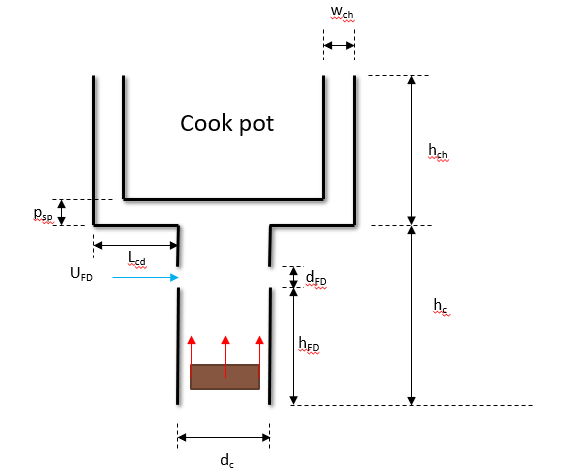
\includegraphics[width=\linewidth]{geometryfrompres.PNG}
	\caption{Figure 1. Cookstove Geometry}
\end{wrapfigure}

\newline

\begin{wraptable}{\linewidth}
	\centering
	\begin{tabular}{||c c||} 
		  \hline
		   Parameter & Variable \\ [0.4ex] 
		    \hline\hline
		     Combustion chamber diameter & d_{c} \\ 
		     Combustion chamber height & h_{c} \\
		     Secondary inlet height & h_{FD} \\
		     Secondary inlet diameter & d_{FD} \\
		     Channel width & w_{ch} \\ [1ex] 
	             Channel height & h_{ch} \\ [1ex]
		     Cone deck length & l_{cd} \\ [1ex]
	             Pot spacing & p_[sp} \\ [1ex]
		     \hline
		     \end{tabular}
		     \newline
		     \newline
		     \caption{Table 1. Geometric Parameters}
	   
\end{wraptable}


\subsection{Mesh}
Mesh details for simulations are defined in the \textit{blockMeshDict} file within the \textit{system} folder of a case directory. Meshes are created by defining hexehedral blocks using vertice definitions.

\subsection{Auxilary Conditions}
Figure 2 below represents the computational domain and will be used to discuss auxilary conditions.

\begin{wrapfigure}{\linewidth}
	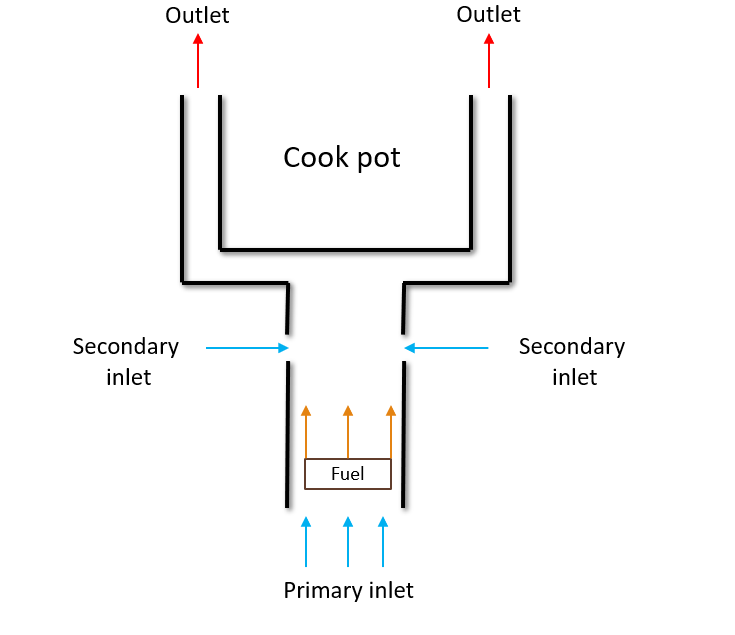
\includegraphics[width=\linewidth]{auxconditions}
	\centering
	\caption{Figure 2. Auxilary Conditions}
	\newline
\end{wrapfigure}

The cookstove primary inlet is modelled as a constant bulk flow velocity of 2.5 m/s of room temperature air composed of 23 percent $O_{2}$ and 77 percent $N_{2}$ by volume; the primary inlet flow velocity was derived based on air mass flow rates predicted by existing experimental results. The fuel zone was assumed to have a constant release of 100 percent methane from each edge. Although this is an inaccurate representation of solid-fuel combustion pertaining to cookstoves, this assumption has less complexity than actual wood combustion, and was deemed reasonable for initial development purposes. The secondary air had the same composition of the primary inlet, however, the bulk flow velocity, although a constant value for an individual simulation, was variable among the different simulation cases; the secondary air flow velocity is the design variable for the optimization and, therefore, is not held constant. For the purposes of this research, the secondary air bulk flow velocity ranged from 25 m/s and 150 m/s; this range was chosen to include the theoretical air-fuel ratio for stoichiometric methane-air combustion. The cookstove outlets were each modelled as atmospheric pressure outlets. The entire domain is assumed to be at a uniform 300 K intially. No slip condition was assigned to all wall boundaries of the cookstove. 


\subsection{Physical Models}
The study depends on an existing OpenFOAM solver called \textit{reactingFoam}, a transient CFD solver that includes combustion chemisty and heat transfer for a compressible fluid flow. The various methods used to model the flow physics are as follows; note, the following information was obtained directly from the OpenFOAM API guide (v1812) \cite{OFapi}.


The reacting flow is assumed to be laminar throughout the computational domain. This was chosen to limit the complexity and runtime of the first attempts of the software.

The thermophysical model used to describe heat transfer due to the reaction is called \textit{psiReactionThermo}, which is a model for a reacting mixture based on the compressibility of the mixture, $\Psi$, given by:

\[$\Psi$ = (RT)^-{1}\] 

Where R is gas constant, and T is the temperature of the mixture. This thermophysical model serves as the basis for many of the OpenFOAM combustion solvers. The mixture is assumed to behave as an ideal gas. The transport model used is based on Sutherland's law, which computes dynamic viscosity, $\mu$, based on the absolute temperature of a mixture T, the Sutherland coefficient $A_{s}$, and Sutherland Temperature $T_{s}$. 
\[$\mu$ = (A_{s}\sqrt{T})/(1 + T_{s}/T)\]

For the purposes of this work, Sutherland coefficient and Sutherland temperature were assigned values of$1.67x10^{-6}$ and $170.67 K$ for each specie in the mixture. Specific heat capacity, $c_{p}$, was computed as a function of mixture temperature T, based on sets of coefficients from NIST JANAF tables for each of the species included \cite{Janaf}. 

\[c_{p} = R((((a_{4}T + a_{3})T + a_{2})T + a_{1})T+ a_{0})\]

Chemistry is modelled using implicit Euler method. The method was chosen to maintain stability for the problem. The flame is assumed to be laminar for the full course of the simulation.


\subsection{Temporal Schemes}
The solver uses the first order implicit Euler method for advancing in time, 

\[(\partial(\phi))/(\partial(t)) = (\phi - \phi^{o})/(\triangle(t))\]

Where $\phi$ represents the variable from the general transport equation, $\triangle$t is the time time step, and $\phi^{o}$ is the general transport variable value from the previous time step.

\subsection{Spatial Schemes}

In order to approximate cell-based quantities at interfaces, a variety of spatial interpolation schemes are required. Gradient terms within the general transport equation were evaluated using second order central differencing. The approximations for gradients of $\phi_{P}$ with neighbors $\phi_{E}$, $\phi_{W}$, $\phi_{N}$, and $\phi_{S}$ are given by,

\[\nabla(\phi_{P}) = (\phi_{E} - \phi_{W})/(\triangle(x)) + (\phi_{N} - \phi_{S})/(\triangle(y)\]


Where $\triangle$x and $\triangle$y are grid spacing in x-coordinate and y-coordinate directions, respectively.

Divergence terms from the general transport equation are approximated using OpenFOAM's \textit{limitedLinear}, which uses a bounded second order central differencing method.

The Laplacian terms, similar to the gradient terms, are approximated using second order central differencing of the form:

\[\nabla^{2}(\phi_{P}) = (\phi_{E}-2\phi_{P} +\phi_{W})/(\triangle(x)^{2}) + (\phi_{N}-2\phi_{P} + \phi_{S})/(\triangle(y)^{2})\]

\subsection{Optimization Algorithm}
The optimization algorithm works to identify an optimal average secondary air flow velocity based on the average cook pot temperature. The optimization process involves the secondary air flow velocity as the single design variable, and the average cook pot temperature as the single performance metric. The flow of the optimization algorithm is presented below in Figure 3. Following the writting of case files, simulations are once again performed and the algorithm is started over once the user is satisfied with the results.

\begin{wrapfigure}{\linewidth}
	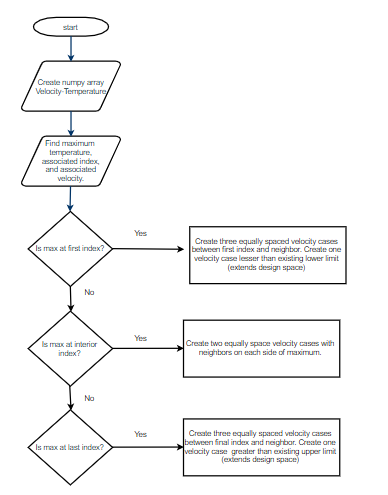
\includegraphics[width=\linewidth]{algorithm.PNG}
	\caption{Figure 3. Optimization Algorithm}
\end{wrapfigure}



The optimization process was designed based on the assumption that the temperature of the cookpot as a function of secondary air flow velocity would behave qualitatively as the ambient temperature varies with respect to the air-fuel ratio for methane-air combustion. For the purpose of illustration, the optimization approach assumes qualitative behavior as depicted by Figure 4.
\newline

\begin{wrapfigure}{\linewidth}
	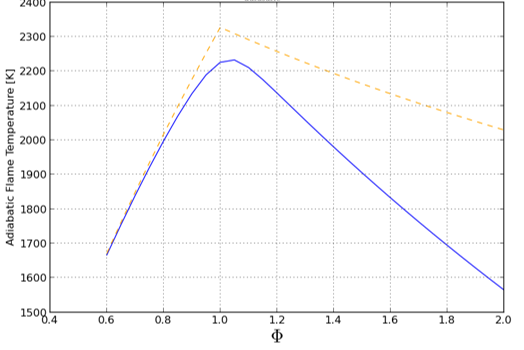
\includegraphics[width=\linewidth]{methair.png}
	\caption{Figure 4. Adiabatic Flame Temperature}
	\newline
\end{wrapfigure}


Given the results of the initial five simulation cases, the optimization algorithm triggers four new cases. Because, theoretically, the optimal flow velocity might exist outside of the range of the first five cases, then the algorithm must have robust functionality. A schematic of the optimization algorithm is presented below in Figure 4.

\section{Implementation}
The StoveOpt software package uses continuous integration by way of the Travis CI tool. Additionally, documentation of the software is available via the link at the master github page (https://github.com/Liam-Cassidy/StoveOpt). Sphinx was used to create the documentation website.

\subsection{Software Layout}
The StoveOpt software contains a collection of modules, which are called within a the main program script. The package contains a test suite compatible with Pytest and an input file which is to be included as a required command line argument. Figure 5 below shows a general structure of the software package.

\begin{wrapfigure}{\linewidth}
	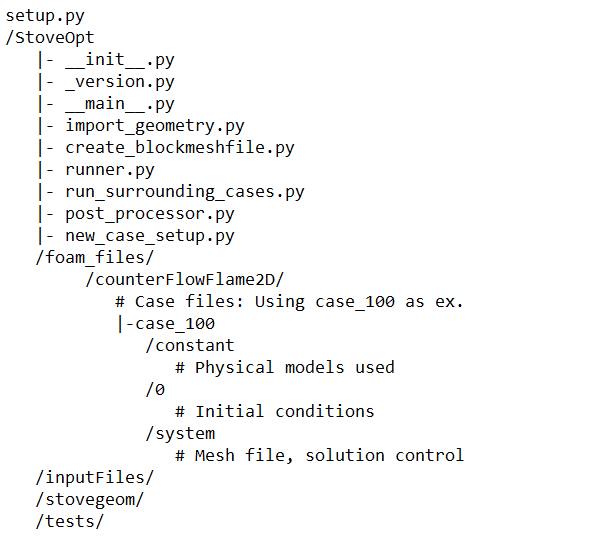
\includegraphics[width=\linewidth]{skeleton.PNG}
	\caption{Figure 5. Package Structure}
\end{wrapfigure}

\subsection{Functionality}
The core functionality of each of the modules within the package are presented below in Table 2. 

\begin{wrapfigure}{\linewidth}
	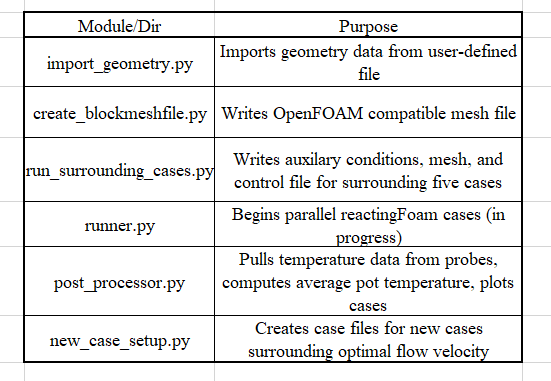
\includegraphics[width=\linewidth]{functionality.PNG}
	\caption{Table 2. Module functionality}
\end{wrapfigure}


\subsection{Dependencies}
The StoveOpt software depends on various python packages. For general navigation and file writing, os, sys, and shutil libraries are required. For array operations, Numpy is required. In order to use the input file and command line arguments, Argparse and Yaml packages are required. matplotlib is used for visualizing data. Lastly, the runner.py module, which is still in development stages, calls upon PyFoam, a python library used to control OpenFOAM simulations. In the current stage of the project, users must have a linux subsystem to run simulations; during development, a Ubuntu terminal was installed for this purpose.


\subsection{Installation}

The software was packaged, and uploaded to PyPI. The package is installable via the pip command. In order to install the current version of the software, simply enter "pip install StoveOpt" from a command line that has pip already installed. 

\subsection{Running the Software}
The current state of the installable package is not capable of excecuting as designed due to complications with packaging. The OpenFOAM input files do not have file type extensions, and were not able to be packaged with the rest of the software. As noted in the $\textit{Installation}$ subsection, the package is installable. However, for the sake of testing the software, the package should be forked from github (https://github.com/Liam-Cassidy/StoveOpt) and cloned locally. The following conversation will assume the software was cloned locally.

To run the software, first, the user must add the filename and directory of the user-defined stove geometry workbook to the \textit{input.yaml} file within the \textit{inputFiles} directory.

\begin{wrapfigure}
	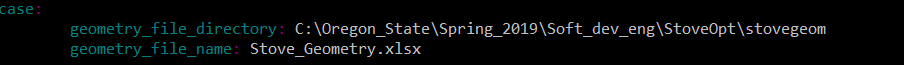
\includegraphics[width=\linewidth]{inputyamlex.PNG}
	\caption{Figure 6. Input Example}
\end{wrapfigure}

Subsequently, users should open a command prompt, and navigate to the StoveOpt directory. The software can then be initiated by calling the main script with the path of the input file as a required argument:

\begin{wrapfigure}{\linewidth}
	
\includegraphics[width=\linewidth]{commandline.PNG}
	\caption{Figure 7. Command Line Instruction}
\end{wrapfigure}

Following the intial run, five OpenFOAM case files will be written. The user then must manually pre-process and enter commands within a Linux-Ubuntu command window. To set up the mesh, users should navigate to a case directory within \textit{/foamfiles/counterFlowFlame2D}; running a \textit{dir} command within a case directory should show \textit{0}, \textit{constant}, and \textit{system} folders. Once at this location, the user should command \textit{blockMesh} in the Ubuntu command window; this calls an OpenFOAM script to create the meshed file. Once the mesh is complete, the user will see a success message, and then should run the command \textit{reactingFoam}. This begins the simulation as dictated by the control files. Running 2-3 cases in parallel is recomended to use computational time economically; multiple cases can be run by openning additional Ubuntu windows, and following the simulation process described above. 
\section{Test Case}
A test case was run in order to evaluate the ability of the software package and understand necessary future work. The inputs used to run the case are presented below.

\subsection{Geometry}

The geometry of the test case is presented below in Table 4.
\newline
\newline

\begin{wraptable}{\linewidth}
	\centering
	\begin{tabular}{||c c c||}
		\hline
		Parameter & Value & Unit \\ [0.4ex]
		\hline\hline
		Combustion chamber diameter & 10 & cm \\
		Combustion chamber height & 29.1 & cm \\
		Secondary inlet height & 15.5 & cm \\
		Secondary inlet diameter & 1 & cm \\
		Channel width & 3 & cm \\
		Channel height & 20 & cm \\
		Cone deck length & 7 & cm \\
		Pot spacing & 3 & cm \\
		\hline
	\end{tabular}
	\newline
	\newline
	\caption{Table 3. Test Case Geometry}
\end{wraptable}


\subsection{Mesh}
A nonuniform mesh was created by assigning three cells within each of the eleven blocks within the domain. The mesh resulted in 560 grid points and 297 cells. An image of the meshed test domain is shown below in Figure 8.
\newline
\begin{wrapfigure}{\linewidth}
	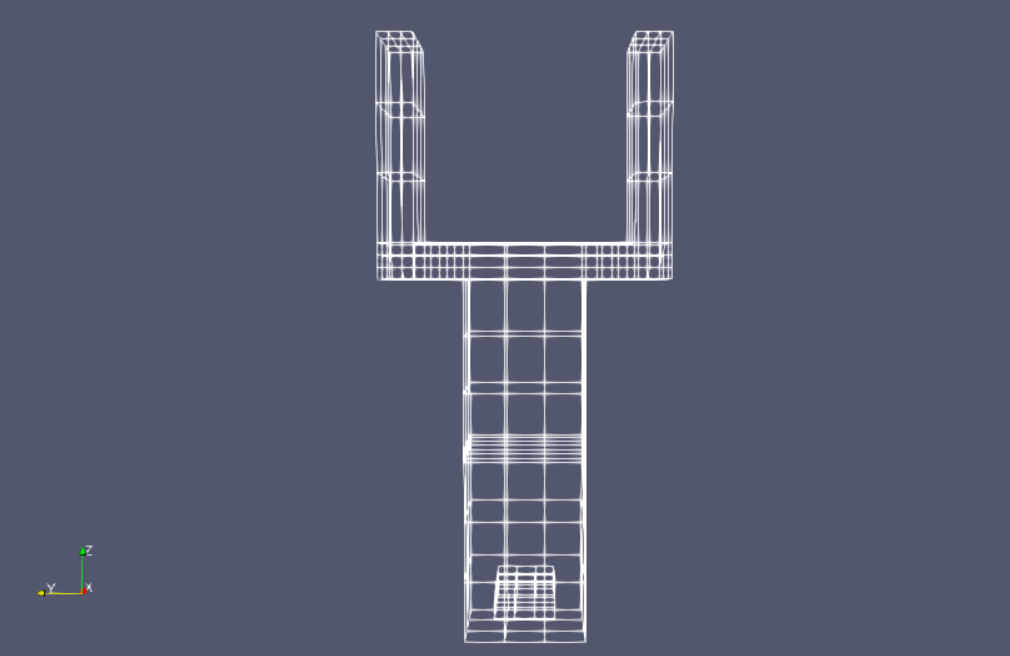
\includegraphics[width=\linewidth]{mesh.PNG}
	\caption{Figure 8. Test Case Mesh}
\end{wrapfigure}


\subsection{Temporal Inputs}
The time step was restricted to $10^{-3}$ seconds to provide reasonable temporal resolution with low computational cost. As discussed previously, the temporal scheme used is implicit, therefore, the solution is bounded regardless of the time step used. Each simulation was run for 10 seconds, with output files written every 0.5 seconds.

\section{Results}
The average pot temperatures for the first five simulations were computed and plotted as shown in Figure 9. The preliminary maximum average pot temperature was about 312 K, and was associated with a secondary air flow velocity of 50 m/s.

\begin{wrapfigure}{\linewidth}
	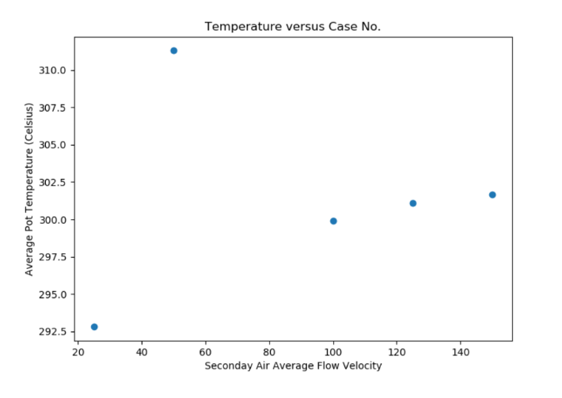
\includegraphics[width=\linewidth]{prelim.png}
	\caption{Figure 9. Pot Temperature vs Flow Velocity: Five Cases}
\end{wrapfigure}


Following the preliminary analysis, the post-processor file was run to identify the max and create the new cases for the purposes of the optimization study. The algorithm correctly identified the flow velocity of 50 m/s as the current maximum, and created four new surrounding cases for the next round of simulaitons. The average pot temperature was plotted once again relative to the secondary air flow velocity; results are shown below in Figure 10.

\begin{wrapfigure}
	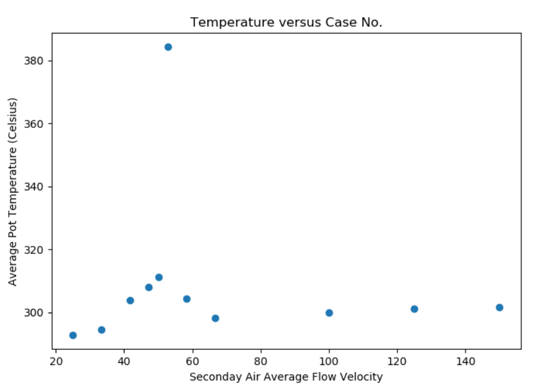
\includegraphics[width=\linewidth]{second.png}
	\caption{Figure 10. Pot Temperature vs Flow Velocity: Nine cases}
\end{wrapfigure}


After post-processing the second batch of simulations, a new optimal air flow rate was identified for the case of 52.8 m/s bulk flow velocity.

\section{Conclusions}
The design curve derived from the test case presented reasonable qualitative results with respect to the expected behavior. Additionally, the algorithm written for the application correctly creates neighboring cases about the optimal design case. The complexities of biomass combustion are not included in the current state of the software. Finally, the cases are computationally expensive due to the nature of the problem, and will require more powerful equipment for most efficient future development.


\section{Future Work}
Future work is essential to provide more robust simulation and optimization, as well as for a stronger optimization algorithm. First, in order to reduce the computational time, the model should be converted to a steady state model with an axisymetric boundary condition along the cookstove centerline. Moreover, a more accurate representation of biomass combustion (both solid and gas phase) is essential for providing a useful software tool for the cookstove development industry. The optimization algorithm should be adapted to include multiple design variables to improve the search within the design space. Lastly, the packaging process needs to be modified to include all of the required OpenFOAM input files.

\section{References}
\bibliography{mybibfile}{}





%% The Appendices part is started with the command \appendix;
%% appendix sections are then done as normal sections
%% \appendix

%% \section{}
%% \label{}

%% References
%%
%% Following citation commands can be used in the body text:
%% Usage of \cite is as follows:
%%   \cite{key}         ==>>  [#]
%%   \cite[chap. 2]{key} ==>> [#, chap. 2]
%%

%% References with BibTeX database:


%% Authors are advised to use a BibTeX database file for their reference list.
%% The provided style file elsarticle-num.bst formats references in the required Procedia style

%% For references without a BibTeX database:

% \begin{thebibliography}{00}

%% \bibitem must have the following form:
%%   \bibitem{key}...
%%

% \bibitem{}

% \end{thebibliography}

\end{document}

%%
%% End of file `ecrc-template.tex'. 
